\PassOptionsToPackage{unicode=true}{hyperref} % options for packages loaded elsewhere
\PassOptionsToPackage{hyphens}{url}
%
\documentclass[]{article}
\usepackage{lmodern}
\usepackage{amssymb,amsmath}
\usepackage{ifxetex,ifluatex}
\usepackage{fixltx2e} % provides \textsubscript
\ifnum 0\ifxetex 1\fi\ifluatex 1\fi=0 % if pdftex
  \usepackage[T1]{fontenc}
  \usepackage[utf8]{inputenc}
  \usepackage{textcomp} % provides euro and other symbols
\else % if luatex or xelatex
  \usepackage{unicode-math}
  \defaultfontfeatures{Ligatures=TeX,Scale=MatchLowercase}
\fi
% use upquote if available, for straight quotes in verbatim environments
\IfFileExists{upquote.sty}{\usepackage{upquote}}{}
% use microtype if available
\IfFileExists{microtype.sty}{%
\usepackage[]{microtype}
\UseMicrotypeSet[protrusion]{basicmath} % disable protrusion for tt fonts
}{}
\IfFileExists{parskip.sty}{%
\usepackage{parskip}
}{% else
\setlength{\parindent}{0pt}
\setlength{\parskip}{6pt plus 2pt minus 1pt}
}
\usepackage{hyperref}
\hypersetup{
            pdftitle={NOAA Storm Data},
            pdfauthor={Shovit Bhari},
            pdfborder={0 0 0},
            breaklinks=true}
\urlstyle{same}  % don't use monospace font for urls
\usepackage[margin=1in]{geometry}
\usepackage{color}
\usepackage{fancyvrb}
\newcommand{\VerbBar}{|}
\newcommand{\VERB}{\Verb[commandchars=\\\{\}]}
\DefineVerbatimEnvironment{Highlighting}{Verbatim}{commandchars=\\\{\}}
% Add ',fontsize=\small' for more characters per line
\usepackage{framed}
\definecolor{shadecolor}{RGB}{248,248,248}
\newenvironment{Shaded}{\begin{snugshade}}{\end{snugshade}}
\newcommand{\AlertTok}[1]{\textcolor[rgb]{0.94,0.16,0.16}{#1}}
\newcommand{\AnnotationTok}[1]{\textcolor[rgb]{0.56,0.35,0.01}{\textbf{\textit{#1}}}}
\newcommand{\AttributeTok}[1]{\textcolor[rgb]{0.77,0.63,0.00}{#1}}
\newcommand{\BaseNTok}[1]{\textcolor[rgb]{0.00,0.00,0.81}{#1}}
\newcommand{\BuiltInTok}[1]{#1}
\newcommand{\CharTok}[1]{\textcolor[rgb]{0.31,0.60,0.02}{#1}}
\newcommand{\CommentTok}[1]{\textcolor[rgb]{0.56,0.35,0.01}{\textit{#1}}}
\newcommand{\CommentVarTok}[1]{\textcolor[rgb]{0.56,0.35,0.01}{\textbf{\textit{#1}}}}
\newcommand{\ConstantTok}[1]{\textcolor[rgb]{0.00,0.00,0.00}{#1}}
\newcommand{\ControlFlowTok}[1]{\textcolor[rgb]{0.13,0.29,0.53}{\textbf{#1}}}
\newcommand{\DataTypeTok}[1]{\textcolor[rgb]{0.13,0.29,0.53}{#1}}
\newcommand{\DecValTok}[1]{\textcolor[rgb]{0.00,0.00,0.81}{#1}}
\newcommand{\DocumentationTok}[1]{\textcolor[rgb]{0.56,0.35,0.01}{\textbf{\textit{#1}}}}
\newcommand{\ErrorTok}[1]{\textcolor[rgb]{0.64,0.00,0.00}{\textbf{#1}}}
\newcommand{\ExtensionTok}[1]{#1}
\newcommand{\FloatTok}[1]{\textcolor[rgb]{0.00,0.00,0.81}{#1}}
\newcommand{\FunctionTok}[1]{\textcolor[rgb]{0.00,0.00,0.00}{#1}}
\newcommand{\ImportTok}[1]{#1}
\newcommand{\InformationTok}[1]{\textcolor[rgb]{0.56,0.35,0.01}{\textbf{\textit{#1}}}}
\newcommand{\KeywordTok}[1]{\textcolor[rgb]{0.13,0.29,0.53}{\textbf{#1}}}
\newcommand{\NormalTok}[1]{#1}
\newcommand{\OperatorTok}[1]{\textcolor[rgb]{0.81,0.36,0.00}{\textbf{#1}}}
\newcommand{\OtherTok}[1]{\textcolor[rgb]{0.56,0.35,0.01}{#1}}
\newcommand{\PreprocessorTok}[1]{\textcolor[rgb]{0.56,0.35,0.01}{\textit{#1}}}
\newcommand{\RegionMarkerTok}[1]{#1}
\newcommand{\SpecialCharTok}[1]{\textcolor[rgb]{0.00,0.00,0.00}{#1}}
\newcommand{\SpecialStringTok}[1]{\textcolor[rgb]{0.31,0.60,0.02}{#1}}
\newcommand{\StringTok}[1]{\textcolor[rgb]{0.31,0.60,0.02}{#1}}
\newcommand{\VariableTok}[1]{\textcolor[rgb]{0.00,0.00,0.00}{#1}}
\newcommand{\VerbatimStringTok}[1]{\textcolor[rgb]{0.31,0.60,0.02}{#1}}
\newcommand{\WarningTok}[1]{\textcolor[rgb]{0.56,0.35,0.01}{\textbf{\textit{#1}}}}
\usepackage{graphicx,grffile}
\makeatletter
\def\maxwidth{\ifdim\Gin@nat@width>\linewidth\linewidth\else\Gin@nat@width\fi}
\def\maxheight{\ifdim\Gin@nat@height>\textheight\textheight\else\Gin@nat@height\fi}
\makeatother
% Scale images if necessary, so that they will not overflow the page
% margins by default, and it is still possible to overwrite the defaults
% using explicit options in \includegraphics[width, height, ...]{}
\setkeys{Gin}{width=\maxwidth,height=\maxheight,keepaspectratio}
\setlength{\emergencystretch}{3em}  % prevent overfull lines
\providecommand{\tightlist}{%
  \setlength{\itemsep}{0pt}\setlength{\parskip}{0pt}}
\setcounter{secnumdepth}{0}
% Redefines (sub)paragraphs to behave more like sections
\ifx\paragraph\undefined\else
\let\oldparagraph\paragraph
\renewcommand{\paragraph}[1]{\oldparagraph{#1}\mbox{}}
\fi
\ifx\subparagraph\undefined\else
\let\oldsubparagraph\subparagraph
\renewcommand{\subparagraph}[1]{\oldsubparagraph{#1}\mbox{}}
\fi

% set default figure placement to htbp
\makeatletter
\def\fps@figure{htbp}
\makeatother


\title{NOAA Storm Data}
\author{Shovit Bhari}
\date{2020-05-07}

\begin{document}
\maketitle

\hypertarget{synopsis}{%
\section{1. Synopsis}\label{synopsis}}

Conduction of this analysis was a part of Coursera Reproducible
Research(Assignment 2), this course is a part of Data Science
Specialization. This project involves exploring the U.S. National
Oceanic and Atmospheric Administration's NOAA Storm Database and its
consequences on both population health and the economy. The
\href{https://d396qusza40orc.cloudfront.net/repdata\%2Fdata\%2FStormData.csv.bz2}{data}
analyzed tracked characteristics of significant storms and weather
events in the United States covered between the years 1950 and November
2011. In the earlier years of the database, there are generally fewer
events recorded, most likely due to a lack of proper records. More
recent years should be considered complete.

This analysis investigates the top severe weather events that were most
harmful to the population health in terms of fatalities and injuries. In
addition, the economic consequence was analyzed by exploring financial
damages on properties and crops.

Here are results of the top severe weather events that cause the most
damages:

\begin{itemize}
\tightlist
\item
  Fatalities: Tornado\\
\item
  Injuries: Tornado\\
\item
  Property Damages: Flood\\
\item
  Crop Damages: Drought
\end{itemize}

\hypertarget{data-processing}{%
\section{2. Data Processing}\label{data-processing}}

\hypertarget{downloading-data}{%
\subparagraph{2.1.1 Downloading Data}\label{downloading-data}}

Download the data from the link provided above. Unzips the data if data
has not been downloaded to the local computer.

\begin{Shaded}
\begin{Highlighting}[]
\KeywordTok{library}\NormalTok{(R.utils)}
\ControlFlowTok{if}\NormalTok{(}\OperatorTok{!}\KeywordTok{file.exists}\NormalTok{(}\StringTok{"./data"}\NormalTok{))\{}\KeywordTok{dir.create}\NormalTok{(}\StringTok{"./data"}\NormalTok{)\}}
\NormalTok{url <-(}\StringTok{"https://d396qusza40orc.cloudfront.net/repdata%2Fdata%2FStormData.csv.bz2"}\NormalTok{)}
\NormalTok{filepath <-}\StringTok{ "./data/StormData.csv.bz2"}
\KeywordTok{download.file}\NormalTok{ (url, filepath)}
\ControlFlowTok{if}\NormalTok{(}\OperatorTok{!}\KeywordTok{file.exists}\NormalTok{(}\StringTok{"./data/StormData.csv"}\NormalTok{))}
\NormalTok{   \{}\KeywordTok{bunzip2}\NormalTok{(}\StringTok{"./data/StormData.csv.bz2"}\NormalTok{, }\StringTok{"./data/StormData.csv"}\NormalTok{)\}}
\end{Highlighting}
\end{Shaded}

\hypertarget{loading-libraries}{%
\subparagraph{2.1.2 Loading Libraries}\label{loading-libraries}}

All the required libraries are loaded.

\begin{Shaded}
\begin{Highlighting}[]
\KeywordTok{library}\NormalTok{(ggplot2)}
\KeywordTok{library}\NormalTok{(dplyr)}
\KeywordTok{library}\NormalTok{(gridExtra)}
\KeywordTok{library}\NormalTok{(formattable)}
\end{Highlighting}
\end{Shaded}

\hypertarget{reading-data}{%
\subparagraph{2.1.3 Reading Data}\label{reading-data}}

Read the data and assign it to the data frame.

\begin{Shaded}
\begin{Highlighting}[]
\NormalTok{data <-}\StringTok{ }\KeywordTok{read.csv}\NormalTok{(}\StringTok{"./data/StormData.csv"}\NormalTok{)}
\end{Highlighting}
\end{Shaded}

\hypertarget{creating-a-subset}{%
\subparagraph{2.2 Creating a subset}\label{creating-a-subset}}

Not all the variables are required for analysis so we have to select
only the required variables.

\begin{Shaded}
\begin{Highlighting}[]
\NormalTok{storm_data <-}\StringTok{ }\KeywordTok{select}\NormalTok{(data, }\KeywordTok{c}\NormalTok{(}\StringTok{"EVTYPE"}\NormalTok{,}\StringTok{"FATALITIES"}\NormalTok{,}\StringTok{"INJURIES"}\NormalTok{,}\StringTok{"PROPDMG"}\NormalTok{, }\StringTok{"PROPDMGEXP"}\NormalTok{,}\StringTok{"CROPDMG"}\NormalTok{,}\StringTok{"CROPDMGEXP"}\NormalTok{)) }
\end{Highlighting}
\end{Shaded}

\hypertarget{health-consequences-fatalities}{%
\subparagraph{2.3.1 Health Consequences
(Fatalities)}\label{health-consequences-fatalities}}

Arrange the fatalities and take a sum by the event type. This provides
us the sum of fatalities caused by different events.

\begin{Shaded}
\begin{Highlighting}[]
\NormalTok{Fatalities <-}\StringTok{ }\KeywordTok{aggregate}\NormalTok{(FATALITIES}\OperatorTok{~}\NormalTok{EVTYPE, }\DataTypeTok{data=}\NormalTok{storm_data, sum)}
\NormalTok{top10_fatalities<-}\StringTok{ }\NormalTok{Fatalities }\OperatorTok\StringTok{ }\KeywordTok{arrange}\NormalTok{(}\KeywordTok{desc}\NormalTok{(FATALITIES)) }\OperatorTok
\StringTok{        }\KeywordTok{top_n}\NormalTok{(}\DecValTok{10}\NormalTok{)}
\end{Highlighting}
\end{Shaded}

\hypertarget{health-consequences-injuries}{%
\subparagraph{2.3.2 Health Consequences
(Injuries)}\label{health-consequences-injuries}}

Arrange the injuries and take a sum by the event type. This provides us
the sum of injuries caused by different events.

\begin{Shaded}
\begin{Highlighting}[]
\NormalTok{Injuries <-}\StringTok{ }\KeywordTok{aggregate}\NormalTok{(INJURIES}\OperatorTok{~}\NormalTok{EVTYPE, }\DataTypeTok{data=}\NormalTok{storm_data, sum)}
\NormalTok{top10_injuries<-}\StringTok{ }\NormalTok{Injuries }\OperatorTok\StringTok{ }\KeywordTok{arrange}\NormalTok{(}\KeywordTok{desc}\NormalTok{(INJURIES)) }\OperatorTok
\StringTok{        }\KeywordTok{top_n}\NormalTok{(}\DecValTok{10}\NormalTok{)}
\end{Highlighting}
\end{Shaded}

\hypertarget{checking-the-unique-values-of-property-damage-exponents}{%
\subparagraph{2.4.1 Checking the unique values of Property Damage
Exponents}\label{checking-the-unique-values-of-property-damage-exponents}}

Property Damage Exponent values in the dataset is assigned as symbols of
``SI Units'' which needs to be identified.

\begin{Shaded}
\begin{Highlighting}[]
\KeywordTok{unique}\NormalTok{(storm_data}\OperatorTok{$}\NormalTok{PROPDMGEXP)}
\end{Highlighting}
\end{Shaded}

\begin{verbatim}
##  [1] K M   B m + 0 5 6 ? 4 2 3 h 7 H - 1 8
## Levels:  - ? + 0 1 2 3 4 5 6 7 8 B h H K m M
\end{verbatim}

\hypertarget{assiging-the-required-values-to-the-exponents.}{%
\subparagraph{2.4.2 Assiging the required values to the
exponents.}\label{assiging-the-required-values-to-the-exponents.}}

Numerical values are assigned to each unique symbols based on their ``SI
Units'' . \href{https://en.wikipedia.org/wiki/Power_of_10}{Wikipedia
Power of 10}

\begin{Shaded}
\begin{Highlighting}[]
\CommentTok{# Assigning values for the property exponent strmdata }
\NormalTok{storm_data}\OperatorTok{$}\NormalTok{PROPEXP[storm_data}\OperatorTok{$}\NormalTok{PROPDMGEXP }\OperatorTok{==}\StringTok{ "M"}\NormalTok{] <-}\StringTok{ }\FloatTok{1e+06}
\NormalTok{storm_data}\OperatorTok{$}\NormalTok{PROPEXP[storm_data}\OperatorTok{$}\NormalTok{PROPDMGEXP }\OperatorTok{==}\StringTok{ ""}\NormalTok{] <-}\StringTok{ }\DecValTok{1}
\NormalTok{storm_data}\OperatorTok{$}\NormalTok{PROPEXP[storm_data}\OperatorTok{$}\NormalTok{PROPDMGEXP }\OperatorTok{==}\StringTok{ "B"}\NormalTok{] <-}\StringTok{ }\FloatTok{1e+09}
\NormalTok{storm_data}\OperatorTok{$}\NormalTok{PROPEXP[storm_data}\OperatorTok{$}\NormalTok{PROPDMGEXP }\OperatorTok{==}\StringTok{ "m"}\NormalTok{] <-}\StringTok{ }\FloatTok{1e+06}
\NormalTok{storm_data}\OperatorTok{$}\NormalTok{PROPEXP[storm_data}\OperatorTok{$}\NormalTok{PROPDMGEXP }\OperatorTok{==}\StringTok{ "0"}\NormalTok{] <-}\StringTok{ }\DecValTok{1}
\NormalTok{storm_data}\OperatorTok{$}\NormalTok{PROPEXP[storm_data}\OperatorTok{$}\NormalTok{PROPDMGEXP }\OperatorTok{==}\StringTok{ "5"}\NormalTok{] <-}\StringTok{ }\FloatTok{1e+05}
\NormalTok{storm_data}\OperatorTok{$}\NormalTok{PROPEXP[storm_data}\OperatorTok{$}\NormalTok{PROPDMGEXP }\OperatorTok{==}\StringTok{ "6"}\NormalTok{] <-}\StringTok{ }\FloatTok{1e+06}
\NormalTok{storm_data}\OperatorTok{$}\NormalTok{PROPEXP[storm_data}\OperatorTok{$}\NormalTok{PROPDMGEXP }\OperatorTok{==}\StringTok{ "4"}\NormalTok{] <-}\StringTok{ }\DecValTok{10000}
\NormalTok{storm_data}\OperatorTok{$}\NormalTok{PROPEXP[storm_data}\OperatorTok{$}\NormalTok{PROPDMGEXP }\OperatorTok{==}\StringTok{ "2"}\NormalTok{] <-}\StringTok{ }\DecValTok{100}
\NormalTok{storm_data}\OperatorTok{$}\NormalTok{PROPEXP[storm_data}\OperatorTok{$}\NormalTok{PROPDMGEXP }\OperatorTok{==}\StringTok{ "3"}\NormalTok{] <-}\StringTok{ }\DecValTok{1000}
\NormalTok{storm_data}\OperatorTok{$}\NormalTok{PROPEXP[storm_data}\OperatorTok{$}\NormalTok{PROPDMGEXP }\OperatorTok{==}\StringTok{ "h"}\NormalTok{] <-}\StringTok{ }\DecValTok{100}
\NormalTok{storm_data}\OperatorTok{$}\NormalTok{PROPEXP[storm_data}\OperatorTok{$}\NormalTok{PROPDMGEXP }\OperatorTok{==}\StringTok{ "7"}\NormalTok{] <-}\StringTok{ }\FloatTok{1e+07}
\NormalTok{storm_data}\OperatorTok{$}\NormalTok{PROPEXP[storm_data}\OperatorTok{$}\NormalTok{PROPDMGEXP }\OperatorTok{==}\StringTok{ "H"}\NormalTok{] <-}\StringTok{ }\DecValTok{100}
\NormalTok{storm_data}\OperatorTok{$}\NormalTok{PROPEXP[storm_data}\OperatorTok{$}\NormalTok{PROPDMGEXP }\OperatorTok{==}\StringTok{ "1"}\NormalTok{] <-}\StringTok{ }\DecValTok{10}
\NormalTok{storm_data}\OperatorTok{$}\NormalTok{PROPEXP[storm_data}\OperatorTok{$}\NormalTok{PROPDMGEXP }\OperatorTok{==}\StringTok{ "8"}\NormalTok{] <-}\StringTok{ }\FloatTok{1e+08}

\CommentTok{# Assigning '0' to invalid exponent strmdata}
\NormalTok{storm_data}\OperatorTok{$}\NormalTok{PROPEXP[storm_data}\OperatorTok{$}\NormalTok{PROPDMGEXP }\OperatorTok\StringTok{ }\KeywordTok{c}\NormalTok{(}\StringTok{"+"}\NormalTok{, }\StringTok{"-"}\NormalTok{, }\StringTok{"?"}\NormalTok{, }\StringTok{""}\NormalTok{)] <-}\StringTok{ }\DecValTok{0}
\end{Highlighting}
\end{Shaded}

\hypertarget{calculating-the-total-property-damage-value}{%
\subparagraph{2.4.3 Calculating the total property damage
value}\label{calculating-the-total-property-damage-value}}

Property damage value is a product of variables PROPDMG and PROPEXP

\begin{Shaded}
\begin{Highlighting}[]
\NormalTok{storm_data}\OperatorTok{$}\NormalTok{PROPDMGVAL <-}\StringTok{ }\NormalTok{storm_data}\OperatorTok{$}\NormalTok{PROPDMG }\OperatorTok{*}\StringTok{ }\NormalTok{storm_data}\OperatorTok{$}\NormalTok{PROPEXP}
\end{Highlighting}
\end{Shaded}

\hypertarget{checking-the-unique-values-of-crop-damage-exponents}{%
\subparagraph{2.5.1 Checking the unique values of Crop Damage
Exponents}\label{checking-the-unique-values-of-crop-damage-exponents}}

Crop Damage Exponent values in the dataset is assigned as symbols of
``SI Units'' which needs to be identified.

\begin{Shaded}
\begin{Highlighting}[]
\KeywordTok{unique}\NormalTok{(storm_data}\OperatorTok{$}\NormalTok{CROPDMGEXP)}
\end{Highlighting}
\end{Shaded}

\begin{verbatim}
## [1]   M K m B ? 0 k 2
## Levels:  ? 0 2 B k K m M
\end{verbatim}

\hypertarget{assiging-the-required-values-to-the-exponents.-1}{%
\subparagraph{2.5.2 Assiging the required values to the
exponents.}\label{assiging-the-required-values-to-the-exponents.-1}}

Numerical values are assigned to each unique symbols based on their ``SI
Units'' . \href{https://en.wikipedia.org/wiki/Power_of_10}{Wikipedia
Power of 10}

\begin{Shaded}
\begin{Highlighting}[]
\CommentTok{# Assigning values for the crop exponent strmdata }
\NormalTok{storm_data}\OperatorTok{$}\NormalTok{CROPEXP[storm_data}\OperatorTok{$}\NormalTok{CROPDMGEXP }\OperatorTok{==}\StringTok{ "M"}\NormalTok{] <-}\StringTok{ }\FloatTok{1e+06}
\NormalTok{storm_data}\OperatorTok{$}\NormalTok{CROPEXP[storm_data}\OperatorTok{$}\NormalTok{CROPDMGEXP }\OperatorTok{==}\StringTok{ "K"}\NormalTok{] <-}\StringTok{ }\DecValTok{1000}
\NormalTok{storm_data}\OperatorTok{$}\NormalTok{CROPEXP[storm_data}\OperatorTok{$}\NormalTok{CROPDMGEXP }\OperatorTok{==}\StringTok{ "m"}\NormalTok{] <-}\StringTok{ }\FloatTok{1e+06}
\NormalTok{storm_data}\OperatorTok{$}\NormalTok{CROPEXP[storm_data}\OperatorTok{$}\NormalTok{CROPDMGEXP }\OperatorTok{==}\StringTok{ "B"}\NormalTok{] <-}\StringTok{ }\FloatTok{1e+09}
\NormalTok{storm_data}\OperatorTok{$}\NormalTok{CROPEXP[storm_data}\OperatorTok{$}\NormalTok{CROPDMGEXP }\OperatorTok{==}\StringTok{ "0"}\NormalTok{] <-}\StringTok{ }\DecValTok{1}
\NormalTok{storm_data}\OperatorTok{$}\NormalTok{CROPEXP[storm_data}\OperatorTok{$}\NormalTok{CROPDMGEXP }\OperatorTok{==}\StringTok{ "k"}\NormalTok{] <-}\StringTok{ }\DecValTok{1000}
\NormalTok{storm_data}\OperatorTok{$}\NormalTok{CROPEXP[storm_data}\OperatorTok{$}\NormalTok{CROPDMGEXP }\OperatorTok{==}\StringTok{ "2"}\NormalTok{] <-}\StringTok{ }\DecValTok{100}
\NormalTok{storm_data}\OperatorTok{$}\NormalTok{CROPEXP[storm_data}\OperatorTok{$}\NormalTok{CROPDMGEXP }\OperatorTok{==}\StringTok{ ""}\NormalTok{] <-}\StringTok{ }\DecValTok{1}

\CommentTok{# Assigning '0' to invalid exponent strmdata}
\NormalTok{storm_data}\OperatorTok{$}\NormalTok{CROPEXP[storm_data}\OperatorTok{$}\NormalTok{CROPDMGEXP }\OperatorTok\StringTok{ }\KeywordTok{c}\NormalTok{(}\StringTok{""}\NormalTok{,}\StringTok{" ?"}\NormalTok{)] <-}\StringTok{ }\DecValTok{0}
\end{Highlighting}
\end{Shaded}

\hypertarget{calculating-the-total-crop-damage-value}{%
\subparagraph{2.5.3 Calculating the total crop damage
value}\label{calculating-the-total-crop-damage-value}}

Crop damage value is a product of variables CROPDMG and CROPEXP

\begin{Shaded}
\begin{Highlighting}[]
\CommentTok{# calculating the crop damage }
\NormalTok{storm_data}\OperatorTok{$}\NormalTok{CROPDMGVAL <-}\StringTok{ }\NormalTok{storm_data}\OperatorTok{$}\NormalTok{CROPDMG }\OperatorTok{*}\StringTok{ }\NormalTok{storm_data}\OperatorTok{$}\NormalTok{CROPEXP}
\end{Highlighting}
\end{Shaded}

\hypertarget{ecomonic-consequences-property-damages}{%
\paragraph{2.6.1 Ecomonic Consequences (Property
Damages)}\label{ecomonic-consequences-property-damages}}

Arrange the property damages and take a sum by the event type. This
provides us the sum of property damages in USD caused by different
events.

\begin{Shaded}
\begin{Highlighting}[]
\NormalTok{prop <-}\StringTok{ }\KeywordTok{aggregate}\NormalTok{(PROPDMGVAL}\OperatorTok{~}\NormalTok{EVTYPE,}\DataTypeTok{data=}\NormalTok{storm_data,}\DataTypeTok{FUN=}\NormalTok{sum,}\DataTypeTok{na.rm=}\OtherTok{TRUE}\NormalTok{)}
\NormalTok{top10_prop<-}\StringTok{ }\NormalTok{prop }\OperatorTok\StringTok{ }\KeywordTok{arrange}\NormalTok{(}\KeywordTok{desc}\NormalTok{(PROPDMGVAL)) }\OperatorTok
\StringTok{        }\KeywordTok{top_n}\NormalTok{(}\DecValTok{10}\NormalTok{)}
\end{Highlighting}
\end{Shaded}

\hypertarget{economic-consequences-crop-damages}{%
\paragraph{2.6.2 Economic Consequences (Crop
Damages)}\label{economic-consequences-crop-damages}}

Arrange the crop damages and take a sum by the event type. This provides
us the sum of crop damages in USD caused by different events.

\begin{Shaded}
\begin{Highlighting}[]
\NormalTok{crop <-}\StringTok{ }\KeywordTok{aggregate}\NormalTok{(CROPDMGVAL}\OperatorTok{~}\NormalTok{EVTYPE,}\DataTypeTok{data=}\NormalTok{storm_data,}\DataTypeTok{FUN=}\NormalTok{sum,}\DataTypeTok{na.rm=}\OtherTok{TRUE}\NormalTok{)}
\NormalTok{top10_crop<-}\StringTok{ }\NormalTok{crop }\OperatorTok\StringTok{ }\KeywordTok{arrange}\NormalTok{(}\KeywordTok{desc}\NormalTok{(CROPDMGVAL)) }\OperatorTok
\StringTok{        }\KeywordTok{top_n}\NormalTok{(}\DecValTok{10}\NormalTok{)}
\end{Highlighting}
\end{Shaded}

\hypertarget{results}{%
\section{3. Results}\label{results}}

\hypertarget{top-10-fatalities}{%
\paragraph{3.1.1 Top 10 Fatalities}\label{top-10-fatalities}}

\begin{Shaded}
\begin{Highlighting}[]
\KeywordTok{formattable}\NormalTok{(top10_fatalities)}
\end{Highlighting}
\end{Shaded}

EVTYPE

FATALITIES

TORNADO

5633

EXCESSIVE HEAT

1903

FLASH FLOOD

978

HEAT

937

LIGHTNING

816

TSTM WIND

504

FLOOD

470

RIP CURRENT

368

HIGH WIND

248

AVALANCHE

224

\hypertarget{top-10-injuries}{%
\paragraph{3.1.2 Top 10 Injuries}\label{top-10-injuries}}

\begin{Shaded}
\begin{Highlighting}[]
\KeywordTok{formattable}\NormalTok{(top10_injuries)}
\end{Highlighting}
\end{Shaded}

EVTYPE

INJURIES

TORNADO

91346

TSTM WIND

6957

FLOOD

6789

EXCESSIVE HEAT

6525

LIGHTNING

5230

HEAT

2100

ICE STORM

1975

FLASH FLOOD

1777

THUNDERSTORM WIND

1488

HAIL

1361

\hypertarget{bar-plot-of-fatalities-and-injuries-as-a-result-of-top-ten-weather-events-in-a-descending-order}{%
\paragraph{3.1.3 Bar plot of fatalities and injuries as a result of top
ten weather events in a descending
order}\label{bar-plot-of-fatalities-and-injuries-as-a-result-of-top-ten-weather-events-in-a-descending-order}}

\begin{Shaded}
\begin{Highlighting}[]
\NormalTok{b1 <-}\StringTok{ }\KeywordTok{ggplot}\NormalTok{(top10_fatalities, }\KeywordTok{aes}\NormalTok{(}\DataTypeTok{x =} \KeywordTok{reorder}\NormalTok{(EVTYPE, FATALITIES), FATALITIES, }\KeywordTok{theme_set}\NormalTok{(}\KeywordTok{theme_classic}\NormalTok{()))) }\OperatorTok{+}\StringTok{ }
\StringTok{        }\KeywordTok{geom_bar}\NormalTok{(}\DataTypeTok{stat =} \StringTok{"identity"}\NormalTok{, }\DataTypeTok{fill =} \StringTok{"cyan4"}\NormalTok{) }\OperatorTok{+}\StringTok{ }
\StringTok{        }\KeywordTok{theme}\NormalTok{(}\DataTypeTok{axis.text.x =} \KeywordTok{element_text}\NormalTok{(}\DataTypeTok{angle =} \DecValTok{0}\NormalTok{, }\DataTypeTok{hjust =} \DecValTok{1}\NormalTok{, }\DataTypeTok{size =} \DecValTok{10}\NormalTok{)) }\OperatorTok{+}\StringTok{ }
\StringTok{        }\KeywordTok{xlab}\NormalTok{(}\StringTok{"Event Type"}\NormalTok{) }\OperatorTok{+}\StringTok{ }\KeywordTok{ylab}\NormalTok{(}\StringTok{"Fatalities"}\NormalTok{) }\OperatorTok{+}\StringTok{ }\KeywordTok{ggtitle}\NormalTok{(}\StringTok{"Total Fatalities by Top 10 Weather Events"}\NormalTok{) }\OperatorTok{+}
\StringTok{        }\KeywordTok{theme}\NormalTok{(}\DataTypeTok{plot.title =} \KeywordTok{element_text}\NormalTok{(}\DataTypeTok{size =} \DecValTok{10}\NormalTok{)) }\OperatorTok{+}\StringTok{ }\KeywordTok{coord_flip}\NormalTok{()}
\end{Highlighting}
\end{Shaded}

\begin{Shaded}
\begin{Highlighting}[]
\NormalTok{b2 <-}\StringTok{ }\KeywordTok{ggplot}\NormalTok{(top10_injuries, }\KeywordTok{aes}\NormalTok{(}\DataTypeTok{x =}  \KeywordTok{reorder}\NormalTok{(EVTYPE, INJURIES), INJURIES, }\KeywordTok{theme_set}\NormalTok{(}\KeywordTok{theme_classic}\NormalTok{()))) }\OperatorTok{+}\StringTok{ }
\StringTok{        }\KeywordTok{geom_bar}\NormalTok{(}\DataTypeTok{stat =} \StringTok{"identity"}\NormalTok{, }\DataTypeTok{fill =}\StringTok{"darkcyan"}\NormalTok{) }\OperatorTok{+}\StringTok{ }
\StringTok{        }\KeywordTok{theme}\NormalTok{(}\DataTypeTok{axis.text.x =} \KeywordTok{element_text}\NormalTok{(}\DataTypeTok{angle =} \DecValTok{0}\NormalTok{, }\DataTypeTok{hjust =} \DecValTok{1}\NormalTok{, }\DataTypeTok{size =} \DecValTok{10}\NormalTok{))}\OperatorTok{+}
\StringTok{        }\KeywordTok{xlab}\NormalTok{(}\StringTok{"Event Type"}\NormalTok{) }\OperatorTok{+}\StringTok{ }\KeywordTok{ylab}\NormalTok{(}\StringTok{"Injuries"}\NormalTok{) }\OperatorTok{+}\StringTok{ }\KeywordTok{ggtitle}\NormalTok{(}\StringTok{"Total Injuries by top 10 Weather Events"}\NormalTok{) }\OperatorTok{+}
\StringTok{        }\KeywordTok{theme}\NormalTok{(}\DataTypeTok{plot.title =} \KeywordTok{element_text}\NormalTok{(}\DataTypeTok{size =} \DecValTok{10}\NormalTok{)) }\OperatorTok{+}\StringTok{ }\KeywordTok{coord_flip}\NormalTok{()}
\end{Highlighting}
\end{Shaded}

\begin{Shaded}
\begin{Highlighting}[]
       \KeywordTok{grid.arrange}\NormalTok{(b1, b2, }\DataTypeTok{nrow =} \DecValTok{2}\NormalTok{, }\DataTypeTok{top =} \StringTok{"Polulation health as a result of the most harmful events"}\NormalTok{)}
\end{Highlighting}
\end{Shaded}

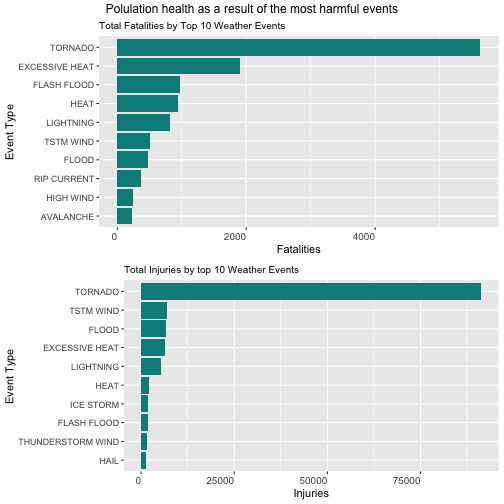
\includegraphics{Project2_files/figure-latex/plot1-1.pdf} \#\#\#\# 3.2.1
Top 10 Property Damages

\begin{Shaded}
\begin{Highlighting}[]
\KeywordTok{formattable}\NormalTok{(top10_prop)}
\end{Highlighting}
\end{Shaded}

EVTYPE

PROPDMGVAL

FLOOD

143779180000

HURRICANE/TYPHOON

69303870000

TORNADO

53783900134

STORM SURGE

43304930000

FLASH FLOOD

15416842262

HAIL

15060160736

HURRICANE

11858970000

TROPICAL STORM

7657980000

WINTER STORM

6557340001

RIVER FLOOD

5105200000

\hypertarget{top-10-crop-damages}{%
\paragraph{3.2.2 Top 10 Crop Damages}\label{top-10-crop-damages}}

\begin{Shaded}
\begin{Highlighting}[]
\KeywordTok{formattable}\NormalTok{(top10_crop)}
\end{Highlighting}
\end{Shaded}

EVTYPE

CROPDMGVAL

DROUGHT

13972566000

FLOOD

5661968450

RIVER FLOOD

5029459000

ICE STORM

5022113500

HAIL

3025954470

HURRICANE

2741910000

HURRICANE/TYPHOON

2607872800

FLASH FLOOD

1421317100

EXTREME COLD

1292973000

FROST/FREEZE

1094086000

\hypertarget{bar-plot-of-property-and-crop-damages-as-a-result-of-top-ten-weather-events-in-a-descending-order}{%
\paragraph{3.2.3 Bar plot of property and crop damages as a result of
top ten weather events in a descending
order}\label{bar-plot-of-property-and-crop-damages-as-a-result-of-top-ten-weather-events-in-a-descending-order}}

\begin{Shaded}
\begin{Highlighting}[]
\NormalTok{h3 <-}\StringTok{ }\KeywordTok{ggplot}\NormalTok{(top10_prop, }\KeywordTok{aes}\NormalTok{(}\DataTypeTok{x =} \KeywordTok{reorder}\NormalTok{(EVTYPE, PROPDMGVAL), PROPDMGVAL, }\KeywordTok{theme_set}\NormalTok{(}\KeywordTok{theme_classic}\NormalTok{()))) }\OperatorTok{+}\StringTok{ }
\StringTok{        }\KeywordTok{geom_bar}\NormalTok{(}\DataTypeTok{stat =} \StringTok{"identity"}\NormalTok{, }\DataTypeTok{fill =} \StringTok{"seagreen1"}\NormalTok{) }\OperatorTok{+}\StringTok{ }
\StringTok{        }\KeywordTok{theme}\NormalTok{(}\DataTypeTok{axis.text.x =} \KeywordTok{element_text}\NormalTok{(}\DataTypeTok{angle =} \DecValTok{0}\NormalTok{, }\DataTypeTok{hjust =} \DecValTok{1}\NormalTok{, }\DataTypeTok{size =} \DecValTok{10}\NormalTok{)) }\OperatorTok{+}\StringTok{ }
\StringTok{        }
\StringTok{        }\KeywordTok{xlab}\NormalTok{(}\StringTok{"Event Type"}\NormalTok{) }\OperatorTok{+}\StringTok{ }\KeywordTok{ylab}\NormalTok{(}\StringTok{"Total Damage (USD)"}\NormalTok{) }\OperatorTok{+}\StringTok{ }\KeywordTok{ggtitle}\NormalTok{(}\StringTok{"Total Property Damage by top 10 Weather Events"}\NormalTok{) }\OperatorTok{+}
\StringTok{        }\KeywordTok{theme}\NormalTok{(}\DataTypeTok{plot.title =} \KeywordTok{element_text}\NormalTok{(}\DataTypeTok{size =} \DecValTok{10}\NormalTok{)) }\OperatorTok{+}\StringTok{ }\KeywordTok{coord_flip}\NormalTok{()}
\end{Highlighting}
\end{Shaded}

\begin{Shaded}
\begin{Highlighting}[]
\NormalTok{h4 <-}\StringTok{ }\KeywordTok{ggplot}\NormalTok{(top10_crop, }\KeywordTok{aes}\NormalTok{(}\DataTypeTok{x =}  \KeywordTok{reorder}\NormalTok{(EVTYPE, CROPDMGVAL), CROPDMGVAL, }\KeywordTok{theme_set}\NormalTok{(}\KeywordTok{theme_classic}\NormalTok{()))) }\OperatorTok{+}\StringTok{ }
\StringTok{        }\KeywordTok{geom_bar}\NormalTok{(}\DataTypeTok{stat =} \StringTok{"identity"}\NormalTok{, }\DataTypeTok{fill =}\StringTok{"seagreen3"}\NormalTok{) }\OperatorTok{+}\StringTok{ }
\StringTok{        }\KeywordTok{theme}\NormalTok{(}\DataTypeTok{axis.text.x =} \KeywordTok{element_text}\NormalTok{(}\DataTypeTok{angle =} \DecValTok{0}\NormalTok{, }\DataTypeTok{hjust =} \DecValTok{1}\NormalTok{, }\DataTypeTok{size =} \DecValTok{10}\NormalTok{)) }\OperatorTok{+}
\StringTok{        }
\StringTok{        }\KeywordTok{xlab}\NormalTok{(}\StringTok{"Event Type"}\NormalTok{) }\OperatorTok{+}\StringTok{ }\KeywordTok{ylab}\NormalTok{(}\StringTok{"Total Damage (USD)"}\NormalTok{) }\OperatorTok{+}\StringTok{ }\KeywordTok{ggtitle}\NormalTok{(}\StringTok{"Total Crop Damage by top 10 Weather Events"}\NormalTok{) }\OperatorTok{+}
\StringTok{        }\KeywordTok{theme}\NormalTok{(}\DataTypeTok{plot.title =} \KeywordTok{element_text}\NormalTok{(}\DataTypeTok{size =} \DecValTok{10}\NormalTok{)) }\OperatorTok{+}\StringTok{ }\KeywordTok{coord_flip}\NormalTok{()}
\end{Highlighting}
\end{Shaded}

\begin{Shaded}
\begin{Highlighting}[]
\KeywordTok{grid.arrange}\NormalTok{(h3, h4, }\DataTypeTok{nrow =} \DecValTok{2}\NormalTok{,}\DataTypeTok{as.table=}\OtherTok{TRUE}\NormalTok{, }\DataTypeTok{top =} \StringTok{"Economic damage as a result of the most harmful events"}\NormalTok{, }\DataTypeTok{padding =} \KeywordTok{unit}\NormalTok{(}\FloatTok{0.5}\NormalTok{, }\StringTok{"line"}\NormalTok{))}
\end{Highlighting}
\end{Shaded}

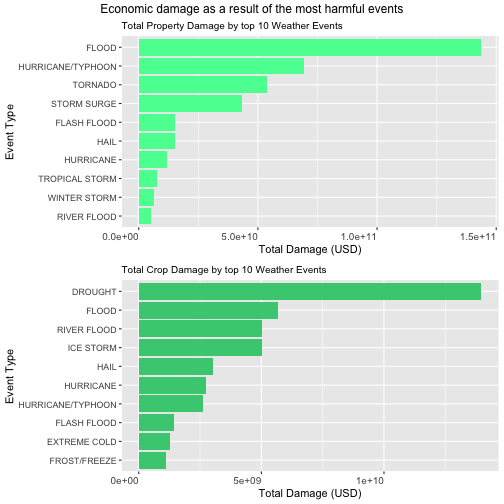
\includegraphics{Project2_files/figure-latex/plot2-1.pdf}

\hypertarget{summary-of-top-events-in-each-category}{%
\subsubsection{3.3 Summary of top events in each
category}\label{summary-of-top-events-in-each-category}}

\begin{itemize}
\tightlist
\item
  Fatalities: Tornado\\
\item
  Injuries: Tornado\\
\item
  Property Damages: Flood\\
\item
  Crop Damages: Drought
\end{itemize}

\end{document}
